%-------------------------------------------------------------------------------
% LATEX TEMPLATE PRESENTATIE
%-------------------------------------------------------------------------------
% Dit template is voor gebruik door studenten van de de bacheloropleiding 
% Informatica van de Universiteit van Amsterdam.
% Voor informatie over presenteren, zie 
%                               https://practicumav.nl/presenteren/index.html
%
%-------------------------------------------------------------------------------
%	PACKAGES EN CONFIGURATIE
%-------------------------------------------------------------------------------
% Gebruik de optie "sidebar" voor toevoeging van een sidebar met inhoudsopgave
% en de optie "dyslexic" voor gebruik van het OpenDyslexic-lettertype
\documentclass[aspectratio=169,classic]{uva-inf-presentation}
\usepackage[english]{babel}
\usepackage{wrapfig}
\usepackage[font=scriptsize,labelfont=bf]{caption}
\usepackage{url}
\usepackage{graphicx}

% Bibliography package
\usepackage[
backend=biber,
style=alphabetic,
sorting=ynt
]{biblatex}
\addbibresource{literature.bib}


% Vul hieronder de gevraagde gegevens in, 
% meerdere auteurs en UvAnetID's gescheiden door een puntkomma 
\title{Dynamic models for multi-variable analysis on stock market behavior} 
\authors{Maarten Peters}
\uvanetids{12754250}
\course{Master Thesis Defence}
\internalSupervisor{Dr Chirstian Rodriguez Rivero}
\externalSupervisor{Dr Julián Antonio Pucheta} 
\programme{Information Studies}
\class{Data Science}

\begin{document}
%-------------------------------------------------------------------------------
%	AUTOMATISCHE SLIDES
%-------------------------------------------------------------------------------
\begin{titelframe}
\titlepage
\end{titelframe}

\begin{titelframe}
\frametitle{Table of contents}
\tableofcontents
\end{titelframe}


%-------------------------------------------------------------------------------
%	PRESENTATIE SLIDES
%-------------------------------------------------------------------------------

% Sample sections
% \section{Eerste sectie}
% \subsection{Eerste subsectie}

% Sample slide
% \begin{frame}
% \frametitle{Titel eerste slide}
% \begin{itemize}
%     \item Test item
%     \item Nieuw test item
% \end{itemize}
% \end{frame}

% INTRO
\section{Introduction}
\begin{frame}
\frametitle{Introduction}
\begin{itemize}
    \item COVID-19 pandemic developments
    \item US \& West Texas Intermediate (WTI) market crash
    \item Economic development
\end{itemize}
\end{frame}

\twocolumn

\begin{frame}
\frametitle{COVID-19 pandemic developments}
\begin{itemize}
    \item Spread of COVID-19
    \item Uncertainty for daily life/businesses
    \item Impact on economic development
    \item Possible government response to mitigate consequences
\end{itemize}
\begin{wrapfigure}{l}{0.4\paperwidth}\centering
    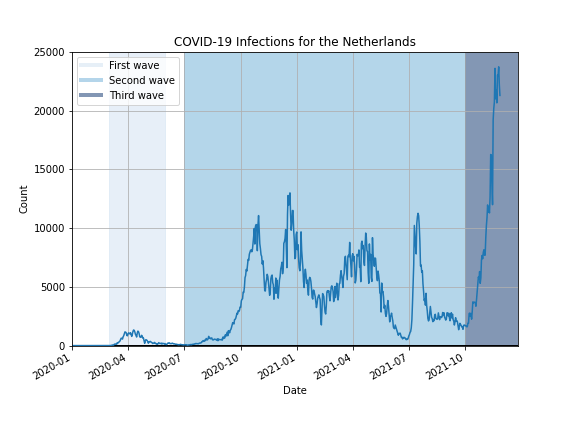
\includegraphics[trim=0cm 1.5cm 0 -3cm, scale=0.4]{images/covid_19_infections_NL.png}
    \caption{COVID-19 Infections in the Netherlands, starting from January 1st, 2020}
\end{wrapfigure}
\end{frame}



\begin{frame}
\frametitle{US \& WTI market crash}
\begin{itemize}
    \item Indicator of crude oil prices
    \item Negative drop in first wave
    \item Proxy of economic development for US
    \item Consequence: US economy crashed, jobs lost, businesses failing
\end{itemize}
\begin{wrapfigure}{l}{0.4\paperwidth}\centering
    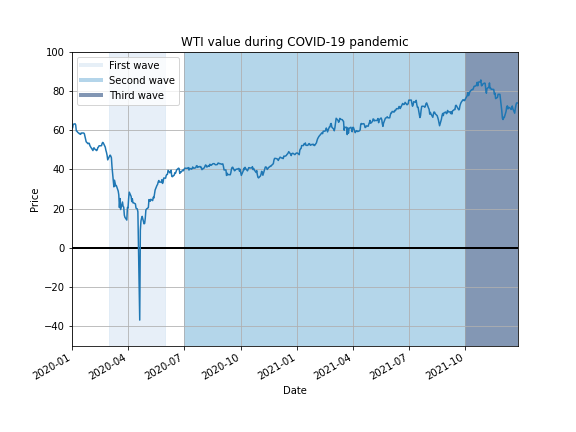
\includegraphics[trim=0cm 1.5cm 0 -3cm, scale=0.4]{images/covid_19_WTI.png}
    \caption{WTI value during COVID-19 pandemic, starting from January 1st, 2020}
\end{wrapfigure}
\end{frame}



\begin{frame}
\frametitle{Economic development \& stock markets}
\begin{itemize}
    \item Stock market indexes (S\&P 500 -> US; AEX25 -> NL) as indicator of economic development
    \item Royal Shell value drops during first wave
    \item Relationship between COVID-19 and stock market indexes
\end{itemize}
\begin{wrapfigure}{l}{0.4\paperwidth}\centering
    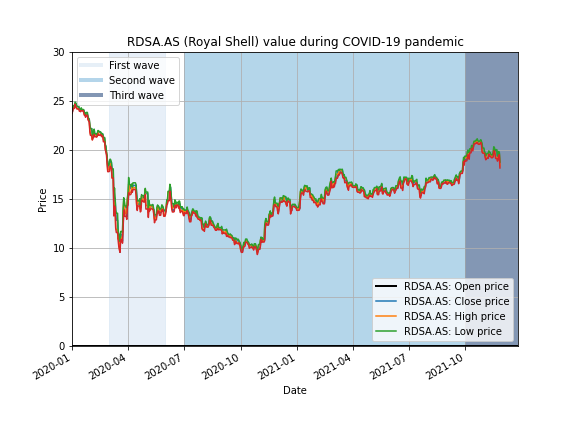
\includegraphics[trim=0cm 1.5cm 0 -3cm, scale=0.4]{images/covid_19_RDSA.png}
    \caption{Royal Shell opening, closing, high and low values during COVID-19 pandemic, starting from January 1st, 2020}
\end{wrapfigure}
\end{frame}

\onecolumn



\subsection{Research questions}
\begin{frame}
\frametitle{Research questions}
\begin{itemize}
    \item[RQ1] \ldots To what extent does the COVID-19 pandemic data influence stock market values?
        \begin{itemize}
            \item Performance of models on short term and long term?
            \item Model performance on similar data?
            \item Generalization over different time-periods?
            \item Which features affect performance to what extent?
        \end{itemize}
    \item[RQ2] \ldots To what extent can machine learning techniques aid in prediction?
\end{itemize}
\end{frame}



% RELATED RESEARCH
\section{Related work}
\begin{frame}
\frametitle{Related work}
\begin{itemize}
    \item COVID-19 pandemic data collections
    \item Stock market \& environmental data 
    \item Existing research
\end{itemize}
\end{frame}

\twocolumn



\subsection{Data}
\begin{frame}
\frametitle{COVID-19 pandemic data}
\begin{itemize}
    \item \textbf{Features:} Infections, deaths, vaccinations \& government measures
    \item Global data by Johns Hopkins University's (JHU) \cite{dong2020interactive} \& University of Oxford \cite{hale2020variation}
    \item Local data by the RIVM
\end{itemize}
\begin{wrapfigure}{l}{0.4\paperwidth}\centering
    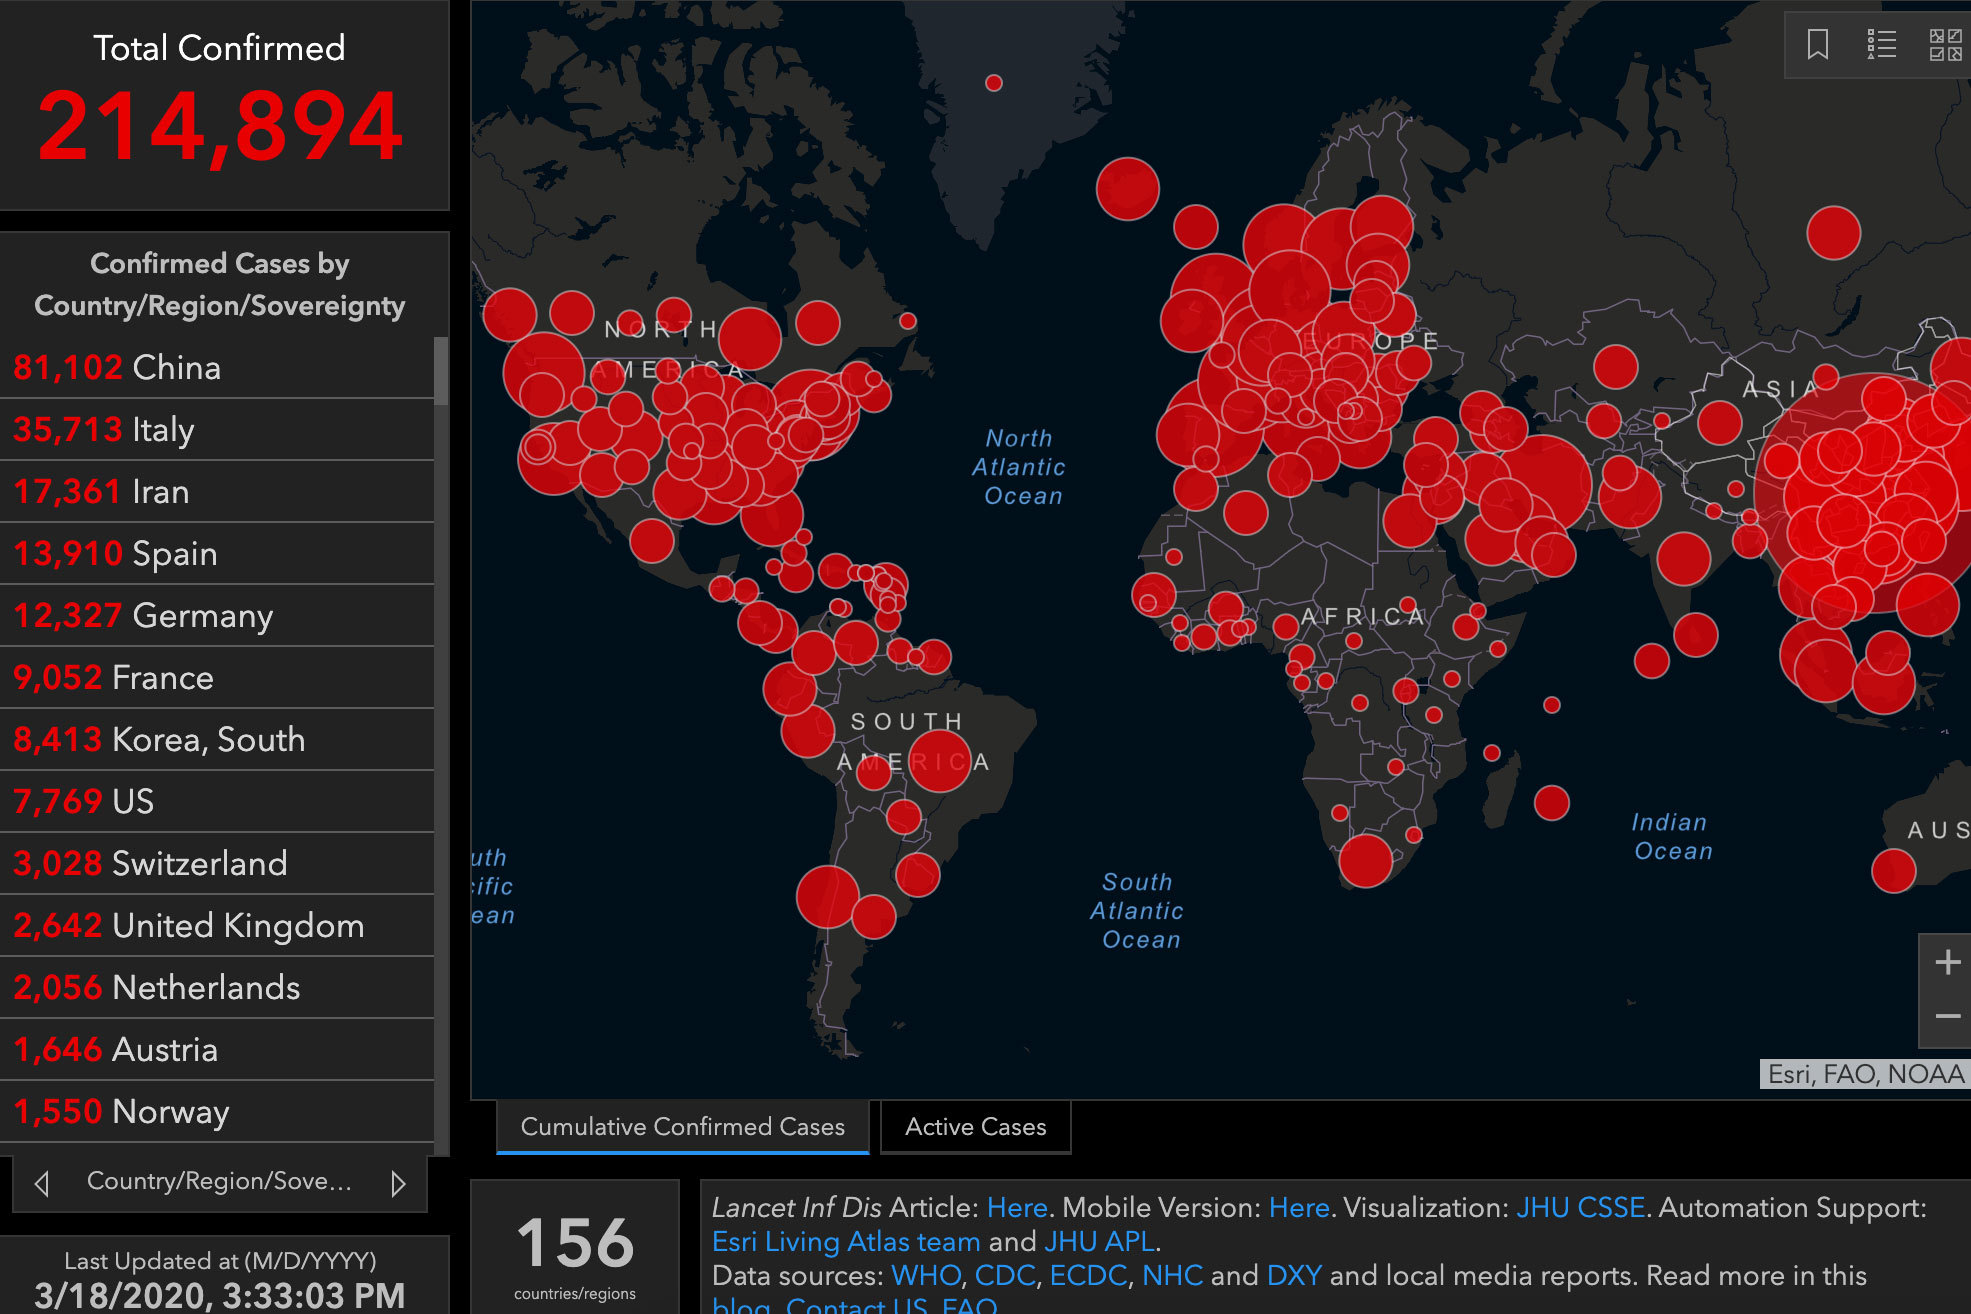
\includegraphics[trim=0cm 0cm 0 -5.5cm, scale=0.3]{images/jhu_samples.jpg}
    \caption{JHU COVID-19 real-time dashboard, source: \href{run:https://www.inquirer.com/health/coronavirus/coronavirus-johns-hopkins-map-world-cases-20200319.html}{The Philidelphia Inquirer}, March 19, 2020}
\end{wrapfigure}
\end{frame}



\begin{frame}
\frametitle{Stock market \& environmental data}
\begin{itemize}
    \item \textbf{Features:} Open, close, high \& low asset prices; traded volume
    \item Collected from Yahoo Finance API \footnote{\href{run:https://pypi.org/project/yfinance/}{Python package \texttt{yfinance}}}
    \item Trading and influence by environment: 
    \begin{itemize}
        \item Weather \cite{hirshleifer2003good}
        \item News \cite{tversky1974judgment, de1985does, veronesi1999stock}
    \end{itemize}
\end{itemize}
\begin{wrapfigure}{l}{0.45\paperwidth}\centering
    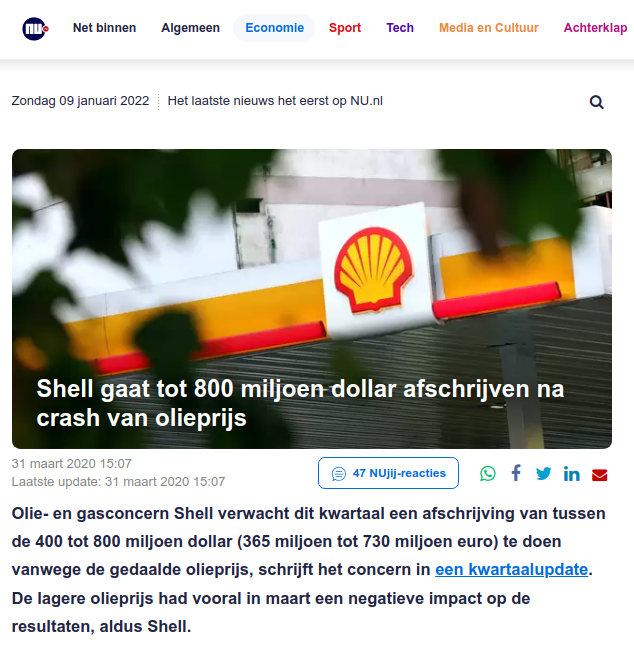
\includegraphics[trim=0cm 0cm 0 -6cm, scale=0.25]{images/shell_news_mar2020.png}
    \caption{Royal Shell amortizes 800 million, source: \href{run:https://www.nu.nl/economie/6041609/shell-gaat-tot-800-miljoen-dollar-afschrijven-na-crash-van-olieprijs.html}{NU.nl}, published March 31st, 2020; taken January 9th, 2021}
\end{wrapfigure}
\end{frame}

\onecolumn



\subsection{Forecasting}
\begin{frame}
\frametitle{Existing research}
\begin{itemize}
    \item Existing models for long-term, needing validation \cite{chudik2020economic, baldwin2020economics, fernandes2020economic}
    \item Historic pandemics offer insight, but model years/decades \cite{osterholm2017preparing, correia1918pandemics, jorda2020longer}
    \item Short-term models show promise on regional level, government measures and with machine learning \cite{zhao2020preliminary, deb2020economic, carpi2021twitter}
\end{itemize}
\end{frame}



% \begin{frame}
% \frametitle{Possible models}
% \begin{itemize}
%     \item Linear regression (LR)\footnote{\href{run:https://scikit-learn.org/}{Python package % \texttt{sklearn} \cite{sklearn2012}}}
%     \item Random Forest Regressor (RFR)\footnotemark[2]
%     \item Auto-regressive integrated moving average (ARIMA)\footnote{Python package % \href{run:https://alkaline-ml.com/pmdarima}{\texttt{pmdarima}: ARIMA estimators for Python}}
%     \item More complex models, such as LSTM, RNN/ANN possible as next step
% \end{itemize}
% \end{frame}



% METHODOLOGY
\section{Methodology}
\begin{frame}
\frametitle{Methodology}
\begin{itemize}
    \item Data: Information gathering
    \item Models: Choosing and fitting models
    \item Evaluation: Model evaluation methods
\end{itemize}
\end{frame}



\subsection{Data}
\begin{frame}
\frametitle{Methodology: Information gathering}
Data for the Netherlands was gathered from \ldots
\begin{itemize}
    \item COVID-19 pandemic: 
    \begin{itemize}
        \item \textbf{JHU}: Vaccinations
        \item \textbf{Oxford}: Government measures \& stringency
        \item \textbf{RIVM}: Infections \& related deaths
    \end{itemize}
    % The Royal Netherlands Meteorological Institute
    \item Environmental data, i.e. weather, from the KNMI, containing:
    \begin{itemize}
        \item Sunshine hours
        \item Precipitation
        \item Wind speeds
    \end{itemize}
\end{itemize}
% All data was cleaned and preprocessed for a daily frequency, where missing figures were zero filled or filled forward.
All feature values were compared between results on our error metric.
\end{frame}

\twocolumn


\onecolumn



\subsection{Models}
\begin{frame}
\frametitle{Models: Choosing and fitting models}
Three models were selected with distinct properties for our data features and compared to a baseline:
\begin{itemize}
    \item \textbf{Linear Regression (LR)}: fits if data is linear and independent
    \item \textbf{Random Forest Regressor (RFR)}: fits if data is non-linear
    \item \textbf{ARIMA}: fits if data is non-linear, but dependent
    \item \textbf{Baseline}: returns the last value of time-series, disregarding all input: $$\hat{Y}_{T+h|T} = Y_T$$
\end{itemize}
Models were fitted automatically with feature selection
\end{frame}



\subsection{Evaluation}
\begin{frame}
\frametitle{Model Evaluation}
Models were compared on mean absolute percentage error (MAPE) for 50 prediction results:
$$\mbox{MAPE} = \frac{100}{n}\sum_{t=1}^n  \left|\frac{A_t-F_t}{A_t}\right|$$
\begin{itemize}
    \item If MAPE >= 1.0: Discard the result, as it constitutes a +100\% error
    \item Baseline error score should be consistent for model comparison
\end{itemize}

\end{frame}

\twocolumn



% RESULTS
\section{Results}
\begin{frame}
\frametitle{Results: Plots 1}
All error scores were compared over different periods, feature sets and daily/weekly frequencies.
\begin{itemize}
    \item Weekly predictions to inconsistent to use
    \item All models struggle to outperform baseline
\end{itemize}
\begin{wrapfigure}{l}{0.4\paperwidth}\centering
    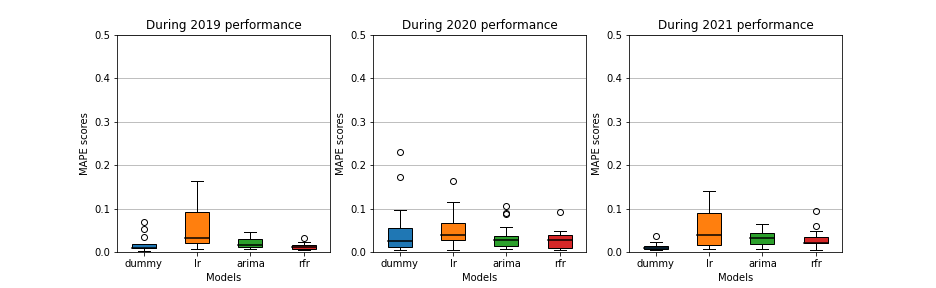
\includegraphics[trim=0cm 0.5cm 0 -6cm, scale=0.25]{images/daily_2019_vs_2020_vs_2021_max_05.png}
    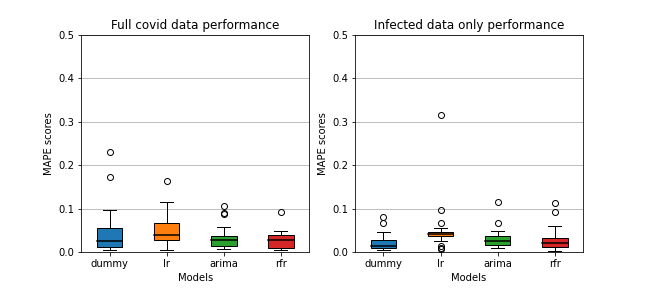
\includegraphics[trim=0cm 0.5cm 0 0cm, scale=0.25]{images/daily_full_covid_data_vs_infected_data_only_max_05.png}
    \caption{\textbf{Top:} Models trained on daily data, split by year, capped at MAPE score <= 0.5 \newline\textbf{Bottom:} Less features favored all models, but no difference from baseline}
\end{wrapfigure}
\end{frame}



\begin{frame}
\frametitle{Results: Plots 2}
Possible issues and remarks:
\begin{itemize}
    \item Sample plots of fitted models showed obvious errors
    \item Error rate consistently decreased with decreased number of features, regardless of pandemic data or weather data
\end{itemize}
\begin{wrapfigure}{l}{0.4\paperwidth}\centering
    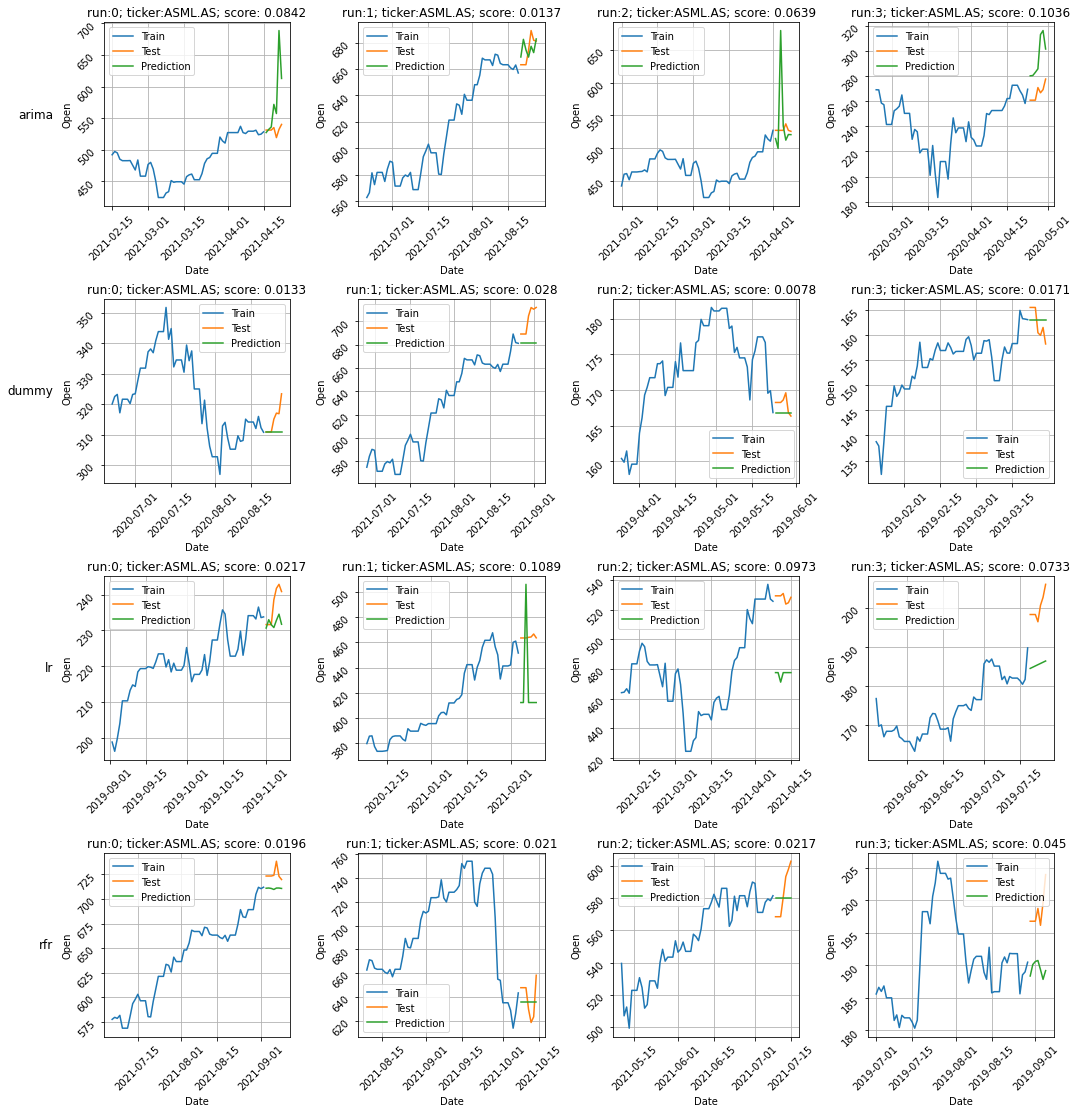
\includegraphics[trim={0cm 20.1cm 9cm -6cm}, scale=0.25, clip]{images/sample_fits_asml.png}
    \caption{Sample predictions for ASML opening price, given access to all data features}
\end{wrapfigure}
\end{frame}

\onecolumn



\begin{frame}
\frametitle{Results: Significance}
Testing for significance of our results, we find that with access to all data features, both state-of-the-art (SOTA) models, ARIMA and RFR, do not significantly ($p < 0.05$) outperform our baseline:

\begin{table}[H]
\begin{tabular}{lllll|}
\cline{4-5}
\multicolumn{3}{l|}{}                                                                                                                        & \multicolumn{2}{l|}{\textbf{Baseline comparison}} \\ \hline
\multicolumn{1}{|l|}{\textbf{Featureset}}                    & \multicolumn{1}{l|}{\textbf{Model}} & \multicolumn{1}{l|}{\textbf{Avg. MAPE}} & \multicolumn{1}{l|}{\textbf{t-stat}}  & \textbf{p} \\ \hline
\multicolumn{1}{|l|}{\multirow{\textbf{All}}} & \multicolumn{1}{|l|}{\textbf{ARIMA}}                      & 0.0302                                  & -0.3735                               & 0.7096     \\ \cline{2-5} 
\multicolumn{1}{|l|}{}                                       & \multicolumn{1}{|l|}{\textbf{RFR}}                        & 0.0234                                  & 0.6711                                & 0.5037     \\ \hline
\multicolumn{1}{|l|}{\multirow{\textbf{None}}}  & \multicolumn{1}{|l|}{\textbf{ARIMA}}                      & 0.0315                                  & -1.7365                               & 0.0856     \\ \cline{2-5} 
\multicolumn{1}{|l|}{}                                       & \multicolumn{1}{|l|}{\textbf{RFR}}                        & 0.0242                                  & -0.5310                               & 0.5966     \\ \hline
\end{tabular}
\caption{Model MAPE score comparison to baseline, for all dataset features and no additional features}
\label{tbl:modelscores}
\end{table}
\end{frame}



% DISCUSSION
\section{Discussion}
\begin{frame}
\frametitle{Discussion}
Possible reasons for inconclusive results:
\begin{itemize}
    \item Proper manual model fitting could be necessary, as domain expertise adds to model accuracy
    \item The efficient market hypothesis (EMH), although debatable, states no individual can outperform the market, given all available information.
    \item The response of stock markets to the precedent of COVID-19 caused speculation/confusion, which subsided over time.
    % \item Our approach using baseline models on highly varied data does not generalize
\end{itemize}
\end{frame}



% CONCLUSION
\section{Conclusion}
\begin{frame}
\frametitle{Conclusion}
\begin{itemize}
    \item[RQ1] \ldots \textit{To what extent does the COVID-19 pandemic data influence stock market values?} \newline
    No conclusive evidence that COVID-19 pandemic data influences stock market values.
    \item[RQ2] \ldots \textit{To what extent can machine learning techniques aid in prediction, given a comparison of baseline models?} \newline
    No conclusive evidence that ARIMA/RFR models aid in prediction, models need manual fitting for proper results.
\end{itemize}
\end{frame}



% QUESTIONS?
\section{Questions}
\begin{frame}
\frametitle{Any questions?}
\begin{itemize}
    \item Thank you for your attention!
    \item ...
    \item This research has been made available on Github: \small{\url{https://github.com/maartenpeters/dynamic-models-for-stock-market-behaviour}}
\end{itemize}
\end{frame}

% ADDITIONAL SLIDES?
\begin{frame}
\frametitle{Additional slides}
\ldots
\end{frame}

\twocolumn

\begin{frame}
\frametitle{Exploratory Data Analysis (EDA) 1}
From EDA we learned that ...
\begin{itemize}
    \item Ordinary least squares regression (OLS) achieves positive $R^2$ scores (>0.7)
    \item Polynomial models improve on LR, but require manual fitting (score >0.9)
    \item Calendar features over complicate models
\end{itemize}
\begin{wrapfigure}{l}{0.45\paperwidth}\centering
    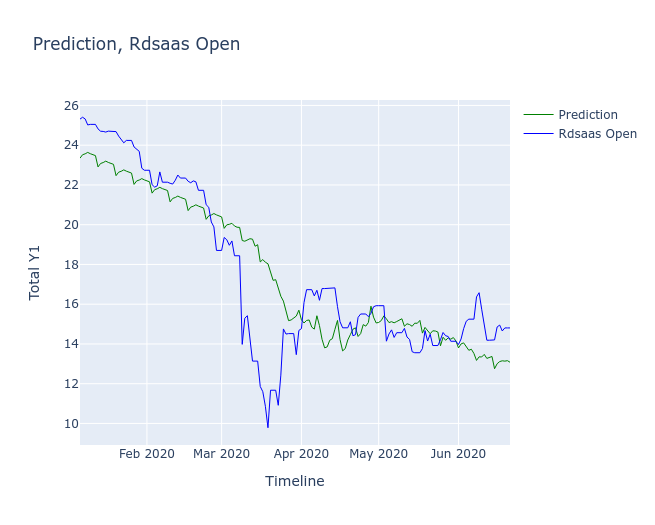
\includegraphics[trim=0cm 0cm 0 -6cm, scale=0.28]{images/EDA.png}
    \caption{OLS fit on RDSA opening prices, with weekday features and COVID-19 infections as input}
\end{wrapfigure}
\end{frame}



\begin{frame}
\frametitle{Exploratory Data Analysis (EDA) 2}
\begin{itemize}
    \item Positive relationship heavily dependent on period of time-series
    \item Correlation scores between RDSA price and COVID-19 infection low, possibly pointing to non-linearity
\end{itemize}
\begin{wrapfigure}{l}{0.45\paperwidth}\centering
    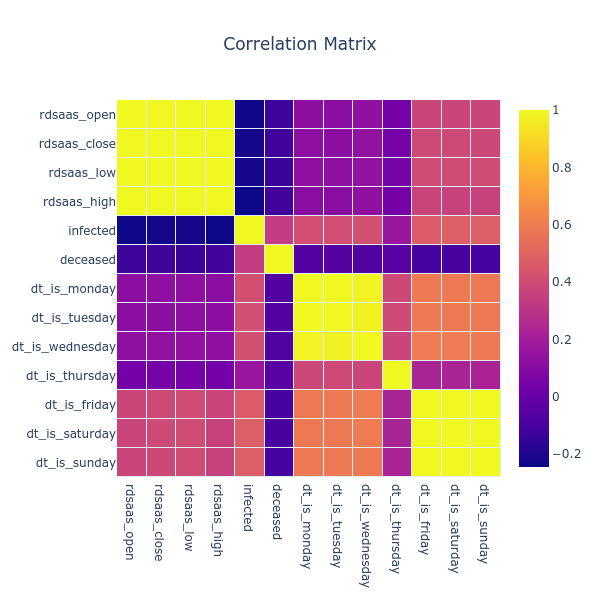
\includegraphics[trim=0cm 0.5cm 0 -6.5cm, scale=0.25]{images/corrplot.png}
    \caption{Heatmap of correlation scores, showing negative correlation between RDSA values and COVID-19 infections and deaths}
\end{wrapfigure}
\end{frame}

\onecolumn

\begin{frame}
\frametitle{Preprocessing and Fitting}
Bofore models were fitted, data was sampled and preprocessed in steps:
\begin{itemize}
    \item Scaling (i.e. between 0 and 1) of all features
    \item Distribution normalized with Yeo-Johnson transformation \cite{yeo2000new}, a variant of Box-Cox allowing for negative values
    \item Second scaling
\end{itemize}
Afterwards, models were trained with recursive feature elimination and five-fold CV on RMSE, with exception for ARIMA
\end{frame}

%-------------------------------------------------------------------------------
%	Additional (practice) questions
%-------------------------------------------------------------------------------

%-------------------------------------------------------------------------------
% Sample defense questions
%-------------------------------------------------------------------------------

% Pick out one or two questions that you consider a nightmare. Write down your answer!

% a)	How well embedded is your research in the existing research? 
% b)	Do you deem your study worthy to be published? What is the scientific value of this all?
% c)	How did you ensure that the results are reproducible? 
% d)	Why did you exclude alternative approaches in favour of your current approach? 
% e)	How sound and complete do you consider your data collection criteria?
% f)	How did you ensure that the annotation was sound and the ground truth reliable?
% g)	How is the choice of your current method justified in light of its performance in previous studies? 
% h)	How did you address reliability and validity concerns in your research? 
% i)	How should we interpret the lack of results in your study? Would you say that this was an inherent risk of the set-up you have chosen? 
% j)	How do you explain the differences between your study and other studies? 
% k)	What would you do differently when you could redo your study? Which limitations % could have been avoided? 
% l)	Why can your study be considered a contribution to the field? 

%-------------------------------------------------------------------------------


% Addtional slides?
\begin{frame}
\frametitle{Additional questions 1}
\begin{itemize}
    \item \textit{How well embedded is your research in the existing research?} \newline
    There is existing research on \ldots
    \begin{itemize}
        \item short term time-series forecasting
        \item long term (economic) effects of (COVID-19) pandemic(s)
        \item stock market indexes as an indicator of economic development
    \end{itemize}
\end{itemize}
\end{frame}

\begin{frame}
\frametitle{Additional questions 2}
\begin{itemize}
    \item \textit{Do you deem your study worthy to be published? What is the scientific value of this all?} \newline
    Yes, although the inconclusive results and possible issues from the discussion do devalue it to some degree. It's scientific value comes primarily from \ldots
    \begin{itemize}
        \item (relatively) new topic of time-series forecasting on stock market values with pandemic data
        \item insight into automated model fitting
    \end{itemize}
\end{itemize}
\end{frame}

\begin{frame}
\frametitle{Additional questions 3}
\begin{itemize}
    \item \textit{How did you ensure that the results are reproducible?} \newline
    \begin{itemize}
        \item All random sampling was seeded consistently
        \item Data gathering and preparation was scripted so all data can be generated
        \item Data sampling, preprocessing, model training and fitting was scripted, so it could be rerun into infinity
        \item Most of the research is documented in the thesis design, EDA and manuscript, along with all code stored in Github.
    \end{itemize}
\end{itemize}
\end{frame}

\begin{frame}
\frametitle{Additional questions 4}
\begin{itemize}
    \item \textit{Why did you exclude alternative approaches in favour of your current approach?} \newline
    With the pandemic being a global event, most of the effort has gone into investigating the effect of variables and well documented models. A different approach would've been to reduce variables and work towards RNN/ANN/LSTM to improve accuracy, but might reduce generalization. As the latter require large amounts of data and fine-tuning, we felt this was unwarranted given the relative novelty of the COVID-19 pandemic.
\end{itemize}
\end{frame}

\begin{frame}
\frametitle{Additional questions 5}
\begin{itemize}
    \item \textit{How sound and complete do you consider your data collection criteria?} \newline
    We believe our data collection and preparation is fully complete. There is room for improvement on implementing it on models, specifically on preprocessing and feature selection/engineering, but this should be model driven.
\end{itemize}
\end{frame}

\begin{frame}
\frametitle{Additional questions 6}
\begin{itemize}
    \item \textit{How did you ensure that the annotation was sound and the ground truth reliable?} \newline
    By putting focus on data gathering and preparation, along with reproducability, we believe our results to be reliable. There is room for improvement on the power of the research, (automatic) (hyper)parameter tuning and quality of the code.
\end{itemize}
\end{frame} 

\begin{frame}
\frametitle{Additional questions 7}
\begin{itemize}
    \item \textit{How is the choice of your current method justified in light of its performance in previous studies?} \newline
    All models are well-documented and have proven their strength and the data also has shown its value in previous studies. The caveat in our study is the automatic model fitting, which did not perform as we hoped, resulting in inconclusive results. Automatic model fitting is to some extent frowned upon, but aides in reproducbility, as rules for fitting are fixed compared to manual intervention.
\end{itemize}
\end{frame} 


\begin{frame}
\frametitle{Additional questions 8}
\begin{itemize}
    \item \textit{How did you address reliability and validity concerns in your research?} \newline
    See slide: Additional questions 3
\end{itemize}
\end{frame} 



\begin{frame}
\frametitle{Additional questions 9}
\begin{itemize}
    \item \textit{How should we interpret the lack of results in your study? Would you say that this was an inherent risk of the set-up you have chosen?} \newline
    Yes, this was an inherent risk of the set-up, but we believe our approach was well considered. This research area was quite novel and had an inherent risk of inconclusive results, given the time, resources and scope of our research. With more time, expertise and an iterative approach on a specific element of our research questions, we might achieve better results.
\end{itemize}
\end{frame} 

 

\begin{frame}
\frametitle{Additional questions 10}
\begin{itemize}
    \item \textit{How do you explain the differences between your study and other studies?} \newline
    Our study differs as it tries to explain variance in stock market values by utilizing event data, specifically COVID-19 pandemic data. Our EDA hinted this might work and related research, although scarce and novel, did support our hypothesis. The difference to our study is we chose to generalize and automate model fitting instead of engineering a specific model for this specific problem.
\end{itemize}
\end{frame} 

\begin{frame}
\frametitle{Additional questions 11}
\begin{itemize}
    \item \textit{What would you do differently when you could redo your study? Which limitations could have been avoided?} \newline
    \begin{itemize}
        \item Focus on reprocubility as a last step
        \item Base our study primarily on a single related paper/dataset and expand the problem space in smaller increments
    \end{itemize}
\end{itemize}
\end{frame} 

\begin{frame}
\frametitle{Additional questions 12}
\begin{itemize}
    \item \textit{Why can your study be considered a contribution to the field?} \newline
    \begin{itemize}
        \item It serves as an insight that modelling time-series on stock market values requires extensive domain knowledge and any gained results in that field is a product of the latter, and not necessarily the model or the data.
        \item It also demonstrates that coincidental correlation does not mean causation or even a relationship in general.
    \end{itemize}
    
\end{itemize}
\end{frame} 

%-------------------------------------------------------------------------------
\end{document}
